\packageentry{tikz}{tikz -- Block diagrams}
\partlabel{Template setup -- styles used by both examples}
\begin{referencecode}
% Graphics packages
\usepackage{graphicx} % Load the graphicx package for including images
\usepackage{float} % Load the float package for improved figure placement
\usepackage{subcaption} % Load the subcaption package for subfigures
\usepackage{wrapfig} % Load the wrapfig package for wrapping text around figures
\usepackage{tikz} % Load the tikz package for creating graphics and diargrams

% Block diagrams package configuration (Tikz)
\usetikzlibrary{shapes, arrows, positioning, decorations.markings, calc}

\newcommand{\midof}[2]{($(#1)!0.5!(#2)$)}

\newlength{\dnd} % default node distance
\setlength{\dnd}{1cm}


\tikzset{
    every picture/.style={
        node distance=\dnd,
    },
    input/.style={
        inner ysep=0.75em,
        inner xsep=0.3em,
    },
    output/.style={
        inner ysep=0.75em,
        inner xsep=0.3em,
    },
    block/.style={
        draw, rectangle, 
        inner ysep=0.75em, 
        inner xsep=1em,
    },
    pickoff/.style={
        circle,
        fill=black,
        minimum size=4pt,
        inner sep=0pt,
    },
    sum/.style={
        draw,
        circle,
        minimum size=1.5em,
        inner sep=0pt,
    },
    plus/.style={
        pos=1,
        inner sep=2pt,
        font=\small,
        node contents={$+$}
    },
    minus/.style={
        pos=1,
        inner sep=2pt,
        font=\small,
        node contents={$-$}
    }
} % Load custom configurations for code formatting
% Loads TikZ and the template styles from:
% Packages/Graphics/package_config.tex
\end{referencecode}
\partlabel{Series blocks}
\begin{referencecode}
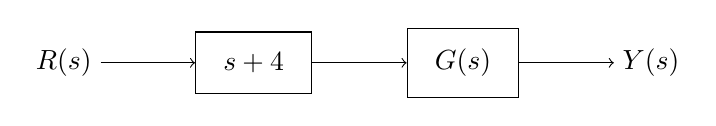
\begin{tikzpicture}[node distance=12mm]
    \node[input] (r) {$R(s)$};
    \node[block,right=of r] (g1) {$s+4$};
    \node[block,right=of g1] (g2) {$G(s)$};
    \node[output,right=of g2] (y) {$Y(s)$};
    \draw[->] (r) -- (g1);
    \draw[->] (g1) -- (g2);
    \draw[->] (g2) -- (y);
\end{tikzpicture}
\end{referencecode}

\begin{figure}[H]\centering

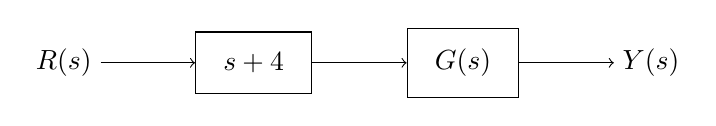
\begin{tikzpicture}[node distance=12mm]
    \node[input] (r) {$R(s)$};
    \node[block,right=of r] (g1) {$s+4$};
    \node[block,right=of g1] (g2) {$G(s)$};
    \node[output,right=of g2] (y) {$Y(s)$};
    \draw[->] (r) -- (g1);
    \draw[->] (g1) -- (g2);
    \draw[->] (g2) -- (y);
\end{tikzpicture}

\caption{Two blocks in series.}\label{fig:series-blocks}
\end{figure}
\verb|right=of g1| uses \texttt{node distance};
\verb|below=15mm of g1| sets a local distance.
\verb|(g1.south)| selects the lower anchor.
The template defines \texttt{input}, \texttt{output}, \texttt{block},
\texttt{sum}, \texttt{pickoff}, \texttt{plus} and \texttt{minus} in
\texttt{Packages/Graphics/package\_config.tex}.
\subsubsection*{Feedback loop}
\phantomsection\label{feedback}
Uses the template styles listed on page~\pageref{tikz}.
\begin{referencecode}
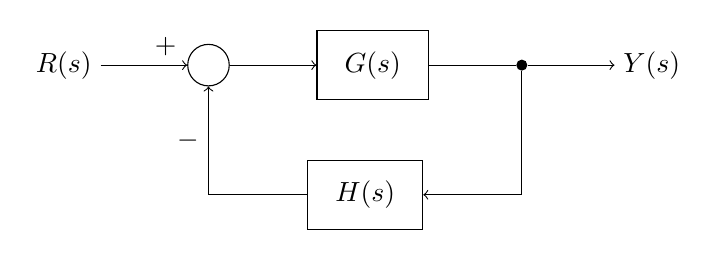
\begin{tikzpicture}[node distance=11mm]
    \node[input] (r) {$R(s)$};
    \node[sum,right=of r] (s) {};
    \node[block,right=of s] (g) {$G(s)$};
    \node[pickoff,right=of g] (p) {};
    \node[output,right=of p] (y) {$Y(s)$};
    \coordinate (mid) at ($(s)!0.5!(p)$);
    \node[block,below=12mm of mid] (h) {$H(s)$};
    \draw[->] (r) -- node[near end,above] {$+$} (s);
    \draw[->] (s) -- (g);
    \draw (g) -- (p);
    \draw[->] (p) -- (y);
    \draw[->] (p) |- (h.east);
    \draw[->] (h.west) -| node[near end,left] {$-$} (s.south);
\end{tikzpicture}
\end{referencecode}

\begin{figure}[H]\centering

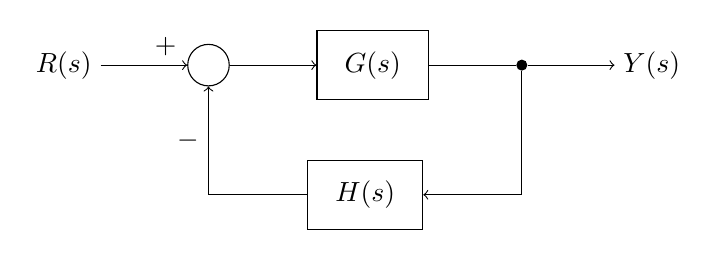
\begin{tikzpicture}[node distance=11mm]
    \node[input] (r) {$R(s)$};
    \node[sum,right=of r] (s) {};
    \node[block,right=of s] (g) {$G(s)$};
    \node[pickoff,right=of g] (p) {};
    \node[output,right=of p] (y) {$Y(s)$};
    \coordinate (mid) at ($(s)!0.5!(p)$);
    \node[block,below=12mm of mid] (h) {$H(s)$};
    \draw[->] (r) -- node[near end,above] {$+$} (s);
    \draw[->] (s) -- (g);
    \draw (g) -- (p);
    \draw[->] (p) -- (y);
    \draw[->] (p) |- (h.east);
    \draw[->] (h.west) -| node[near end,left] {$-$} (s.south);
\end{tikzpicture}

\caption{Negative-feedback block diagram.}\label{fig:feedback-loop}
\end{figure}

\subsubsection*{Coordinates and scaling}
\begin{referencecode}
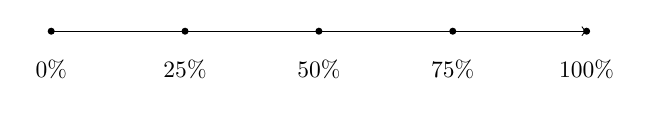
\begin{tikzpicture}[scale=0.85,transform shape]
    \coordinate (s) at (0,0);
    \coordinate (p) at (8,0);
    \coordinate (quarter) at ($(s)!0.25!(p)$);
    \coordinate (centre) at ($(s)!0.50!(p)$);
    \coordinate (threequarters) at ($(s)!0.75!(p)$);
    \draw[->] (s) -- (p);
    \foreach \point/\percent in
        {s/0,quarter/25,centre/50,threequarters/75,p/100} {
        \fill (\point) circle (1.5pt);
        \node[below=3mm] at (\point) {\percent\%};
    }
\end{tikzpicture}
\end{referencecode}

\begin{figure}[H]\centering

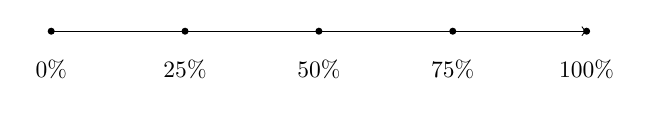
\begin{tikzpicture}[scale=0.85,transform shape]
    \coordinate (s) at (0,0);
    \coordinate (p) at (8,0);
    \coordinate (quarter) at ($(s)!0.25!(p)$);
    \coordinate (centre) at ($(s)!0.50!(p)$);
    \coordinate (threequarters) at ($(s)!0.75!(p)$);
    \draw[->] (s) -- (p);
    \foreach \point/\percent in
        {s/0,quarter/25,centre/50,threequarters/75,p/100} {
        \fill (\point) circle (1.5pt);
        \node[below=3mm] at (\point) {\percent\%};
    }
\end{tikzpicture}

\caption{Interpolated coordinates at a scale of 0.85.}
\end{figure}
\verb|--| draws a straight line; \verb+|-+ goes vertically then
horizontally; \verb+-|+ does the reverse.
\texttt{calc} enables interpolation between nodes.
\texttt{transform shape} scales the node text and shapes too.

